In this section, the goal is to discuss potential threats about the two macro-areas covered by this report:
communication (specifically VANETs) and the perception system,
giving a comprehensive overview of the potential threats and the
countermeasures that can be adopted to mitigate them, focussing on remote attacks.
Since there are two crucial aspects of the AVs, the potential threats are numerous and varied.
The multitude of technologies involved in these two areas makes the AVs vulnerable to a wide range of attacks,
decreasing the threshold of security.
Attackers can exploit these vulnerabilities to compromise the safety and functionality of AVs, posing significant risks to passengers, pedestrians, and other road users.
Since now cars are connected to the internet, there is no need to be physically close to the car to exploit these vulnerabilities and this expands the attack surface drastically.
In the past decade (2010 onward), nearly 79.6\% of all automotive attacks have been
remote attacks\cite{cybersec}.

\subsection{General}\label{subsec:communication-system}

This section highlights various attacks, possible tempering and threats that affect the security services in general regarding
the CIA triad.
It is important to mention that the CIA triad is a model designed to guide policies for information security, and in the list below, some techniques cannot be present.

\paragraph{Attack on Confidentiality}
\begin{enumerate}
    \item \textbf{Eavesdropping}: Intercepts confidential information, such as user identity and location.
    \item \textbf{Traffic Analysis}: Analyzes message transmission patterns to extract sensitive information.
    \item \textbf{Man-in-the-Middle}: Intercepts and alters messages between communicating vehicles.
    \item \textbf{Social Engineering}: Distracts and exploits drivers to gain access to confidential information.
    \item \textbf{Sybil Attack}: Uses multiple fake identities to mislead vehicles and compromise confidentiality.
    \item \textbf{GPS Spoofing}: Creates false GPS information, compromising location confidentiality.
\end{enumerate}

\paragraph{Attack on Data Integrity}
\begin{enumerate}
    \item \textbf{Masquerading}: Uses valid credentials to broadcast false messages.
    \item \textbf{Replay}: Repeats or delays transmissions, complicating emergency responses.
    \item \textbf{Message Tampering}: Modifies messages to influence driving behavior.
    \item \textbf{Illusion}: Generates misleading traffic warnings based on malicious data.
    \item \textbf{Node Impersonation}: Uses a valid user ID to impersonate another user, compromising the integrity of communications.
    \item \textbf{Key/Certificate Replication}: Uses duplicates to create confusion, affecting data authenticity and integrity.
\end{enumerate}

\paragraph{Attack on Availability}
\begin{enumerate}
    \item \textbf{Denial-of-Service}: Blocks vehicle communication, disrupting operations; can occur as distributed denial of service (DDoS)\cite{sontakke2022impact}.
    \item \textbf{Jamming}: Uses strong signals to disrupt communication channels, critical for safety applications.
    \item \textbf{Malware}: Penetrates OBUs, RSUs or other system component leading to system malfunctions.
    \item \textbf{Broadcast Tampering}: Untrustworthy vehicles alter or replicate messages, hiding critical safety information.
    \item \textbf{Black-hole}: Malicious nodes receive but do not forward packets, obstructing communication.
    Another version is the \textit{Gray-hole} that selectively drops only some packets.
\end{enumerate}


To deepen the knowledge about other specific techniques for attacking and potential countermeasures, a specific evaluation
can be found in~\cite{simulation-attacks-vanets, sheikh2019comprehensive, macena2023cybersecurity}.

\begin{table}[h]
    \centering
    \begin{tabular}{|l|l|l|}
        \hline
        \textbf{Attack} & \textbf{Compromised} & \textbf{Countermeasures} \\ \hline
        DOS & A & Signature-based authentication technique \ref{subsec:intrusion-detection-and-prevention-systems} \\ \hline
        Jamming & A & Direct-sequence spread spectrum (DSSS\cite{wang2022when}) \\ \hline
        Malware & A & Reliable hardware and digital signature of software \\ \hline
        Broadcast tampering & I, A & Non-repudiation mechanism may exist \\ \hline
        Black-hole, gray-hole & A & Reliable hardware and digital signature of software \\ \hline
        Greedy behavior & A & Use intrusion detection systems (IDSs) \\ \hline
        Spamming & C, A & Reliable hardware and digital signature of software \\ \hline
        Eavesdropping & C, I & Exploit physical layer security protocols \\ \hline
        Traffic analysis & C & Encryption techniques \\ \hline
        Man-in-the-middle & C, I, A & Robust authentication technique (E.g. CA) \\ \hline
    \end{tabular}
    \label{tab:Summary of Attacks and Countermeasures}
\end{table}
A = Availability, AU = Authentication, C = Confidentiality, I = Integrity
from\cite{sheikh2019comprehensive}.

\subsection{VANETs specific}\label{subsec:v2x-communication-and-network}

In this section, the focus is on the communication system, specifically on the VANETs.
In this case, some countermeasures are presented to mitigate the threats that affect the security services in VANETs, in particular the location privacy and related info.
Some of the main countermeasures, with benefits and limitations, are presented and discussed.


below\cite{macena2023cybersecurity}.

\subsubsection{Pseudonym Change and Silent Periods}
Dividing road networks into observed and unobserved zones allows vehicles to change pseudonyms and behavior, such as altering speeds and directions in unobserved zones.
This, combined with random silent periods in vehicle-to-vehicle (V2V) communication, reduces the risk of tracking and identity linking.
However, this approach can lead to privacy loss and computational strain for certain vehicles, particularly in V2I (vehicle-to-infrastructure) interactions, where more complex tasks are required.

\begin{enumerate}
    \item \textbf{Key Features}:
    \begin{enumerate}
        \item Road networks divided into observed/unobserved zones.
        \item Vehicles in unobserved zones change pseudonyms, directions, and speeds.
        \item Random silent periods in V2V communications to unlink identities.
    \end{enumerate}
    \item \textbf{Limitations}: Navigation group leaders privacy and computational overhead in V2I applications.
\end{enumerate}

\subsubsection{Cryptographic MIX-Zone (CMIX)}
Here, RSUs (Roadside Units) provide cryptographic keys to vehicles, enabling secure pseudonym exchanges in encrypted zones.
This method strengthens privacy, but the high costs of the required hardware and the complexity of managing pseudonym certification represent significant hurdles, particularly when applied on a larger scale.
\begin{enumerate}
    \item \textbf{Key Features}:
    \begin{enumerate}
        \item RSUs provide vehicles with cryptographic keys.
        \item Pseudonym exchange in encrypted mixing zones.
        \item Possible pseudonym certification through authorities.
        \item Optional use of hardware security modules (HSMs).
    \end{enumerate}
    \item \textbf{Challenges}: High hardware costs and managing pseudonym certification.
\end{enumerate}

\subsubsection{K-Anonymity}
A trusted server anonymizes data, and location information is shared only if enough vehicles are present nearby, making individual tracking more difficult.
This technique is scalable and can be adjusted based on vehicle density, making it well-suited for dynamic traffic conditions.
\begin{enumerate}
    \item \textbf{Key Features}:
    \begin{enumerate}
        \item Trusted server anonymizes data via cloaking.
        \item Location shared only if \emph{K} vehicles are nearby.
    \end{enumerate}
    \item \textbf{Advantages}: Scalable and customizable based on vehicle density.
\end{enumerate}

\subsubsection{Dynamic Change MAC/PHY}
Periodic swapping of these addresses complicates tracking efforts.
Cryptographic key exchanges ensure that address changes are secure, although this approach requires careful management of the cryptographic process to maintain seamless communication.
\begin{enumerate}
    \item \textbf{Key Features}:
    \begin{enumerate}
        \item Periodic MAC/PHY address swapping.
        \item Cryptographic key exchange during address changes.
    \end{enumerate}
    \item \textbf{Advantages}: Makes vehicle tracking harder.
\end{enumerate}

\subsubsection{Density-Based Location Privacy (DLP)}
Offers protection by changing pseudonyms based on the number of surrounding vehicles.
In high-traffic areas, this method enhances privacy, but determining the optimal conditions for triggering pseudonym changes can be a challenge,
particularly in environments with rapidly shifting traffic densities.
\begin{enumerate}
    \item \textbf{Key Features}:
    \begin{enumerate}
        \item Pseudonym change occurs with \emph{k} neighboring nodes.
        \item Improved privacy in high-traffic areas.
    \end{enumerate}
    \item \textbf{Challenges}: Dynamic pseudonym change thresholds.
\end{enumerate}

The integration of pseudonyms, cryptographic techniques, dynamic address changes, and density-based strategies offers a comprehensive framework
for improving location privacy, however, practical implementation requires careful consideration of the associated costs and complexities\cite{macena2023cybersecurity}.


\subsection{Perception System}\label{subsec:perception-system}

The perception system in AVs is responsible for collecting and processing data from various sensors to understand the vehicle's surroundings.
The data collected by the perception system is crucial for making informed decisions and coordinating the vehicle's actuators in a safe and efficient manner.
However, since it is composed by a multitude of sensors, the perception system is a subsystem where the attack surface is huge\ref{fig:sensors-2}.
In this section, some main issues about the perception system will be presented and discussed, focusing on the potential threats and the countermeasures that can be adopted to mitigate them\cite{sensors}.

As mentioned, some sensors are \textit{LiDAR}, \textit{radar}, \textit{cameras}, and \textit{ultrasonic sensors}, to perceive and interpret their surroundings accurately.
For their nature, it is challenging preventing from common attacks like spoofing and jamming.
Sensor spoofing involves introducing false data into the sensor systems, while jamming overwhelms the sensors with noise, disrupting their normal functioning.

Through such manipulation, attackers can deceive the vehicle's control systems, causing misinterpretations of the environment.
For example, projecting fake obstacles might cause unnecessary braking, while concealing real obstacles could lead to collisions.
These manipulations result in erratic driving behavior.
In cases of jamming, AVs may become \textit{careless} to their surroundings, resulting in dangerous situations due to the absence of reliable sensor input\cite{durlik2022cybersecurity}.

\begin{figure}[!htb]
    \centering
    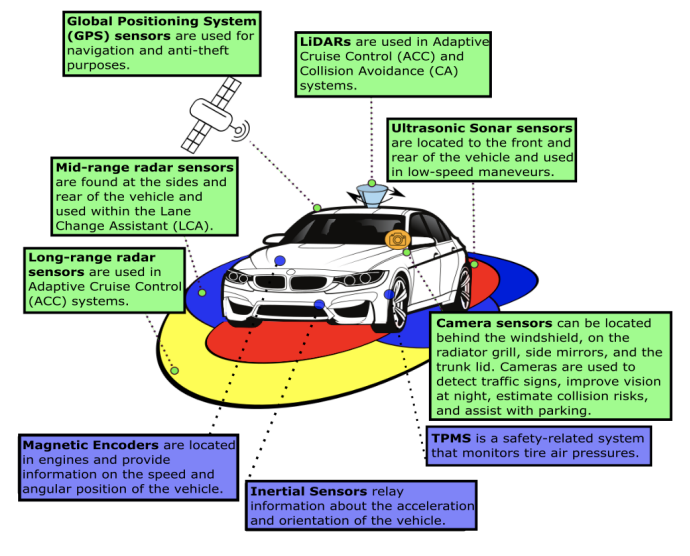
\includegraphics[width=0.7\linewidth]{figures/sensors}
    \caption{Main sensors used in AVs from \cite{sensors}}
    \label{fig:sensors-2}
\end{figure}

What emerges from the literature is that the perception system is a critical component of AVs, mainly every sensor can be a potential target for cyber-attacks using the techniques mentioned above.
From LiDAR, Ultrasonic Sensor, Camera, Radar, GPS, that are the most common sensors used is AVs, to the Tire Pressure sensors are all potential targets\cite{sensors}.


\paragraph{Countermeasures}

Given the complexity of autonomous vehicle perception systems, they can easily become a target for attacks.
The current approach acknowledges this vulnerability, which is challenging to fully eliminate.
Instead, the focus is shifting towards recognizing the stimuli detected by these systems and determining whether they are legitimate or not.
As highlighted in the machine learning/AI section\ref{subsec:artificial-intelligence}, machine learning algorithms—particularly those for anomaly detection—are being employed to identify and respond to irregularities in sensor data.
Another possible countermeasure is sensor fusion, which involves cross-referencing data from multiple sensors.
This technique helps to provide more accurate measurements and enables more stable decision-making and reactions.

However, while machine learning offers new avenues for detecting and mitigating these attacks, it introduces new challenges in terms of legal and ethical considerations.
Since the focus is not on these aspects but in the technical ones, it is essential to consider the forensic implications
of these algorithms\cite{durlik2022cybersecurity, cybersecurity2022forensics} and possible research for the future to eliminate these vulnerabilities.

\begin{figure}[!htb]
    \centering
    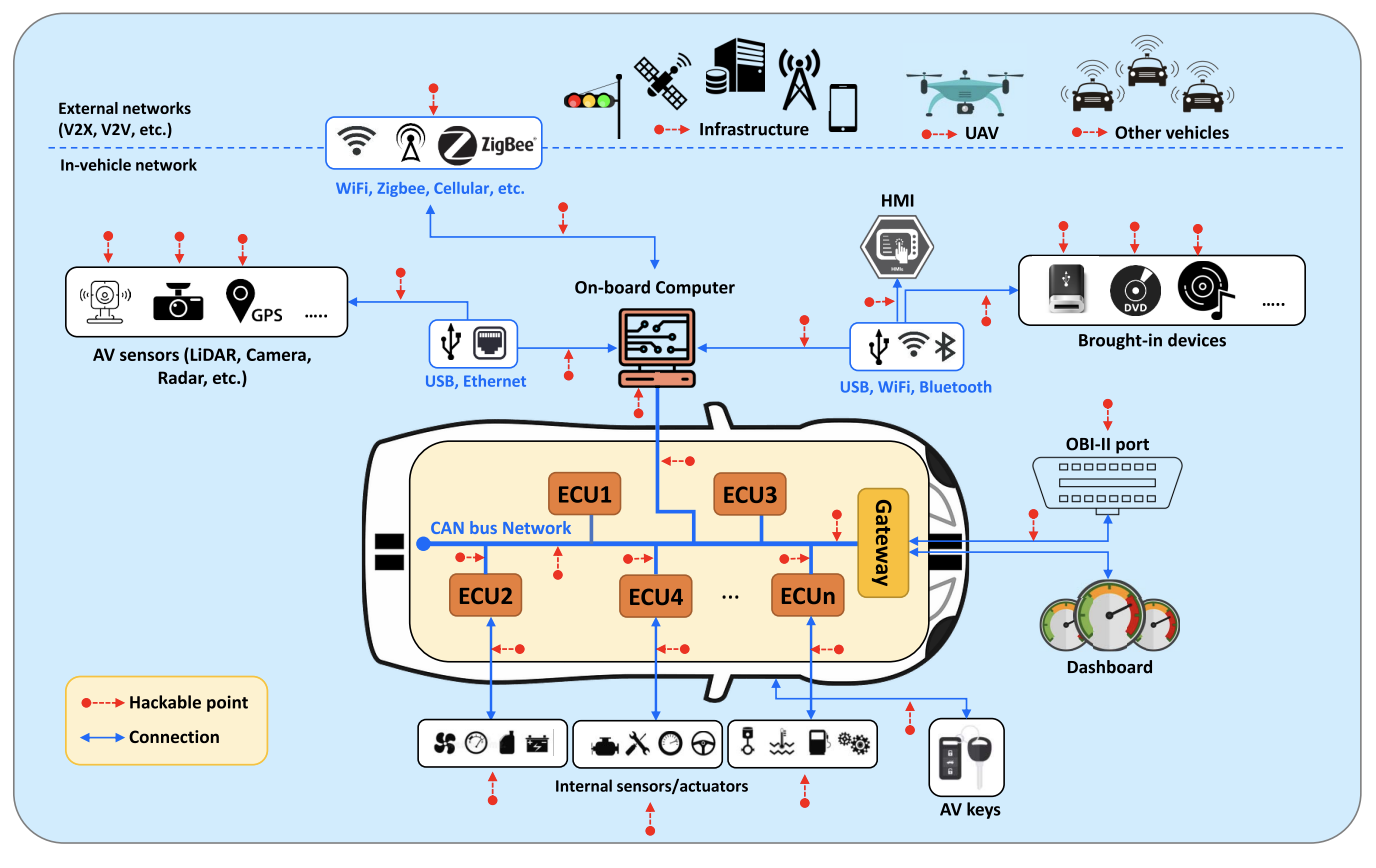
\includegraphics[width=0.7\linewidth]{figures/vectors}
    \caption{Main attack vectors from \cite{bendiab2023autonomous}}
    \label{fig:attack-vectors}
\end{figure}